\documentclass[10pt,a4paper]{article}

\usepackage[margin=0.55in, top=0.52in, bottom=0.52in]{geometry}
\usepackage{fontspec}
\setmainfont{Times New Roman}
\newfontfamily\khmerfont{Segoe UI}

\usepackage{amsmath,amssymb,amsfonts}
\usepackage{booktabs}
\usepackage{tabularx}
\usepackage{array}
\usepackage[table]{xcolor}
\usepackage{hyperref}
\usepackage{fancyhdr}
\usepackage{titlesec}
\usepackage{tcolorbox}
\usepackage{enumitem}
\usepackage{graphicx}
\usepackage{ragged2e}
\usepackage{float}
\usepackage{makecell}

% ── Color Palette ─────────────────────────────────────────────────────────────
\definecolor{NavyBlue}{RGB}{12, 44, 98}       % Primary Blue
\definecolor{Teal}{RGB}{20, 110, 120}         % Secondary Teal
\definecolor{DarkSlate}{RGB}{33, 37, 41}      % Charcoal Slate
\definecolor{LightGrey}{RGB}{248, 249, 251}   % Background tint
\definecolor{BorderGrey}{RGB}{218, 222, 228}  % Border line
\definecolor{Emerald}{RGB}{25, 135, 84}       % Green
\definecolor{RowTint}{RGB}{245, 248, 253}     % Table row tint

\hypersetup{
    colorlinks=true,
    linkcolor=NavyBlue,
    citecolor=Teal,
    urlcolor=NavyBlue,
    pdftitle={Nowcasting Inflation via Daily Web Scraping Price},
    pdfauthor={TAING Korngmeng}
}

% ── Header and Footer ─────────────────────────────────────────────────────────
\pagestyle{fancy}
\fancyhf{}
\fancyhead[L]{\footnotesize\color{gray}Project Progress · Nowcasting Inflation via Daily Web Scraping Price}
\fancyhead[R]{\footnotesize\color{gray}GDDE / MEF \& ITC}
\fancyfoot[L]{\footnotesize\color{gray}Author: TAING Korngmeng (Data Science, AMS/ITC)}
\fancyfoot[R]{\footnotesize\color{gray}Page \thepage}
\renewcommand{\headrulewidth}{0.4pt}
\renewcommand{\footrulewidth}{0.4pt}

% ── Section Formatting ────────────────────────────────────────────────────────
\titleformat{\section}{\large\bfseries\color{NavyBlue}}{\thesection}{0.5em}{}[\titlerule]
\titleformat{\subsection}{\normalsize\bfseries\color{Teal}}{\thesubsection}{0.4em}{}
\titleformat{\subsubsection}{\small\bfseries\color{DarkSlate}}{\thesubsubsection}{0.3em}{}

\titlespacing*{\section}{0pt}{4pt}{2pt}
\titlespacing*{\subsection}{0pt}{3pt}{1pt}
\titlespacing*{\subsubsection}{0pt}{2pt}{1pt}

\begin{document}

% =============================================================================
% TITLE & HEADER
% =============================================================================

\begin{center}
    {\large\bfseries\color{Teal} Project Progress}\\[0.08cm]
    {\LARGE\bfseries\color{NavyBlue} Nowcasting Inflation via Daily Web Scraping Price}\\[0.05cm]
    {\footnotesize Author: TAING Korngmeng \quad|\quad Host: GDDE / MEF \quad|\quad Institution: ITC (AMS) \quad|\quad Date: September 2026}
\end{center}

\vspace{-0.10cm}

% =============================================================================
% 1. OBJECTIVE
% =============================================================================
\section*{1. Objective}

\begin{itemize}[noitemsep,topsep=1.5pt,leftmargin=*]
    \item \textbf{Build an Automated Data Infrastructure and Monitoring System:} Set up an automated data pipeline and database to collect, store, and continuously monitor prices.
    \item \textbf{Calculate CPI for Inflation Nowcasting Using Machine Learning Model:} Apply an economic formula to compute daily price relatives, and use regularized Ridge regression modeling to nowcast inflation ahead of the official monthly release.
    \item \textbf{Build a Decision-Support Dashboard:} Develop an interactive dashboard that presents daily CPI results and inflation for easy monitoring.
\end{itemize}

\vspace{-0.05cm}

% =============================================================================
% 2. ARCHITECTURE
% =============================================================================
\section*{2. Architecture}

\begin{figure}[H]
    \centering
    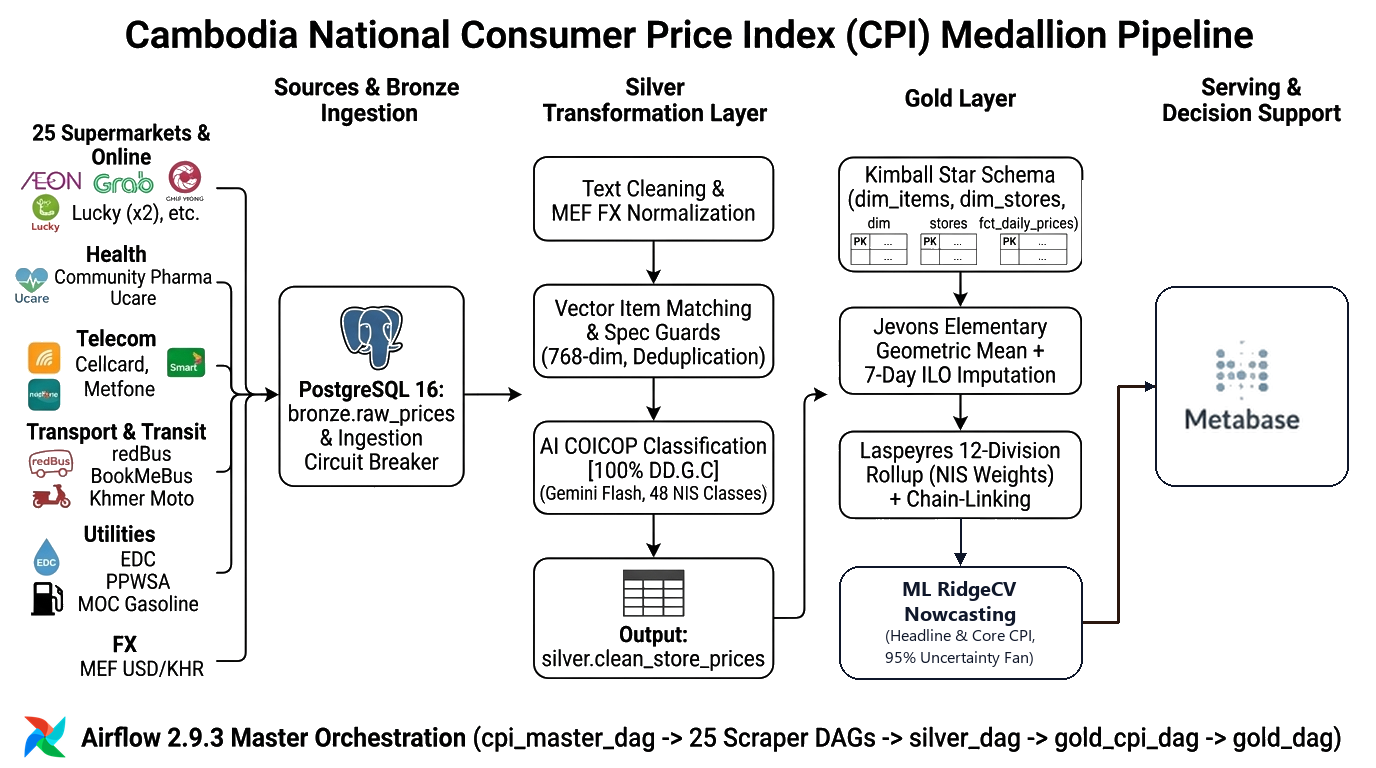
\includegraphics[width=0.62\textwidth]{thesis/images/cpi_architecture_clean.png}
    \vspace{-0.15cm}
    \caption{End-to-End System Architecture: Web Scraping, Medallion Pipeline \& Dashboard.}
    \label{fig:arch}
\end{figure}

\vspace{-0.30cm}
\subsection*{Technology Stack}

\noindent
\footnotesize
\renewcommand{\arraystretch}{0.80}
\begin{tabularx}{\textwidth}{@{}>{\bfseries}p{5.5cm}X@{}}
\toprule
\rowcolor{NavyBlue!15} Component / Pipeline Layer & Technology Stack \\ \midrule
Data Ingestion \& Scraping & Python \\ \addlinespace
\rowcolor{RowTint} Database and Storage & PostgreSQL 16 \\ \addlinespace
Orchestration & Apache Airflow \\ \addlinespace
\rowcolor{RowTint} Data Transformation & dbt Core \\ \addlinespace
AI Product Classifications & Gemini AI \\ \addlinespace
\rowcolor{RowTint} Dashboard and Monitoring & Metabase \\ \addlinespace
System Container & Docker \\ \bottomrule
\end{tabularx}

\vspace{0.05cm}

% =============================================================================
% 3. DATA COLLECTION
% =============================================================================
\section*{3. Data Collection}

\noindent
\footnotesize
\renewcommand{\arraystretch}{0.80}
\begin{tabularx}{\textwidth}{@{}>{\bfseries}p{5.5cm}X@{}}
\toprule
\rowcolor{NavyBlue!15} Data Source & Description \\ \midrule
AEON Online Cambodia & Supermarket \\ \addlinespace
\rowcolor{RowTint} DeliShop Asia Phnom Penh & Supermarket \\ \addlinespace
GrabMart (Lucky Supermarket, Chip Mong) & Supermarket \\ \addlinespace
\rowcolor{RowTint} L192 Online Marketplace & Footwear \& Homeware \\ \addlinespace
Community Pharmacy \& Ucare Pharmacy & Healthcare \& Pharmaceutical Goods \\ \addlinespace
\rowcolor{RowTint} Khmer24 \& Realestate.com.kh & Urban Residential Apartment, House Rentals \\ \addlinespace
redBus \& BookMeBus Transit & Bus \& Travel Transport \\ \addlinespace
\rowcolor{RowTint} Cellcard, Smart Axiata, Metfone & Mobile Plan and Wi-Fi \\ \addlinespace
Tela Khmer & Gasoline \\ \addlinespace
\rowcolor{RowTint} dataEF API & Exchange Rate \\ \addlinespace
Sokha, Hyatt, Bayon BKK & Restaurant and Hotel \\ \bottomrule
\end{tabularx}

\clearpage

% =============================================================================
% 4. METHODOLOGY
% =============================================================================
\section*{4. Methodology}

\subsection*{Stage 1: Web Scraping Layer}
\noindent\textbf{Automated Daily Collection:} Every morning at 08:00 AM, the system automatically collects prices across 11 key stores and services in Cambodia.\\[0.1cm]
\noindent\textbf{How We Collect Prices:}
\begin{itemize}[noitemsep,topsep=1pt,leftmargin=*]
    \item \textbf{Direct Store APIs:} Connects directly to the backend of online supermarkets (AEON, DeliShop) and apps (L192, BookMeBus) to download product lists and prices quickly without loading heavy web pages.
    \item \textbf{Browser Disguise (\texttt{curl\_cffi}):} Sends fast automated requests that look like a real Google Chrome browser so store security systems (like Cloudflare) do not block our computer.
    \item \textbf{Invisible Browser (Playwright):} If a website blocks direct requests with security checks (like 403 Forbidden), the system automatically opens an invisible browser to load the page and read the prices like a real user.
    \item \textbf{Public Pages \& Feeds:} Reads apartment rental listings from Khmer24, fuel prices from the Tela Khmer public channel (translating Khmer numbers 0--9), and official daily exchange rates from the Ministry of Economy and Finance (MEF).
    \item \textbf{Safety \& Backup Rules:} Pauses 1 second between requests so we do not slow down store websites, and sends an alert if 0 products are found so bad data is never saved.
\end{itemize}

\subsection*{Stage 2: Bronze Layer (Raw Lake Ingestion)}
\noindent\textbf{Database Table:} \texttt{bronze.raw\_prices}
\begin{itemize}[noitemsep,topsep=1pt,leftmargin=*]
    \item \textbf{What it does:} Acts as an immutable, append-only raw data repository preserving the exact raw data as fetched from the web.
    \item \textbf{Stored Fields:} \texttt{store\_id}, \texttt{source\_name}, \texttt{item\_description\_raw}, \texttt{price}, \texttt{currency}, \texttt{source\_url}, \texttt{scraped\_at}, \texttt{batch\_id}.
\end{itemize}

\subsection*{4.3 Data Cleaning, Matching, and AI Classification}
\noindent\textbf{Database Table:} \texttt{silver.standardized\_prices}\\[0.05cm]
The Silver Layer transforms messy raw scraped microdata into standardized economic items through 3 core jobs:
\begin{center}
    \textbf{[Raw Scrape] $\longrightarrow$ 1. Clean Data $\longrightarrow$ 2. Match Product $\longrightarrow$ 3. Classify Basket $\longrightarrow$ [Clean Silver Item]}
\end{center}

\subsubsection*{4.3.1 Data Cleaning \& Standardization}
\begin{itemize}[noitemsep,topsep=1pt,leftmargin=*]
    \item \textbf{Clean product names and text:} Remove HTML tags, special characters, promotional words (SALE, HOT DEAL, 50\% OFF), unnecessary text, and convert text to lowercase.
    \item \textbf{Convert Khmer numerals $\rightarrow$ Arabic numerals:} Convert Khmer digits (e.g., {\khmerfont ៥០០} $\rightarrow$ 500) for consistent processing.
    \item \textbf{Convert USD $\rightarrow$ KHR:} Convert dual currencies using the official MEF daily exchange rate.
    \item \textbf{Standardize weight, volume, and package units:} Convert package sizes into standard metric units (e.g., 500g to 0.5kg, 1500ml to 1.5L).
    \item \textbf{Calculate unit prices (KHR/kg, KHR/L, etc.):} Compute unit price ($P_{\text{unit}} = \text{Price in KHR} / \text{Normalized Metric}$) to fairly compare different product sizes.
\end{itemize}

\subsubsection*{4.3.2 Product Matching (4-Level Waterfall)}
\noindent
Connects identical products across different stores and tracks them day-after-day:
\begin{itemize}[noitemsep,topsep=1pt,leftmargin=*]
    \item \textbf{Level 1 --- Barcode (GTIN / EAN):} Matches the exact same item across different stores (e.g., AEON $\leftrightarrow$ DeliShop) using global standard barcodes.
    \item \textbf{Level 2 --- Store ID + SKU (Composite Key):} Remembers the item day-after-day within the same store (AEON yesterday $\leftrightarrow$ AEON today).
    \begin{itemize}[noitemsep]
        \item \textit{What is SKU?} A unique Stock Keeping Unit code assigned by a store, extracted directly from product URLs or store APIs.
        \item \textit{The Problem:} Different stores reuse the same SKU number (e.g., SKU 100 at AEON is Beef Curry, but at DeliShop is Fruit Syrup).
        \item \textit{The Solution (Composite Key):} Combines (\texttt{store\_id}, \texttt{sku}) so each store catalog remains strictly isolated.
        \item \textit{Learn Once, Cache Forever:} The first time an item is scraped, it is saved into canonical tables. On daily scrapes, the system instantly recognizes it without re-matching.
    \end{itemize}
    \item \textbf{Level 3 --- Exact Text Matching:} Links different stores selling the exact same product when no barcode is available.
    \begin{itemize}[noitemsep]
        \item \textit{When Triggered?} When no universal barcode is provided and the store SKU is unseen.
        \item \textit{Why Needed?} Different stores assign different SKUs to the exact same item (e.g., AEON SKU 123 vs. AryStore SKU 999 for "Samsung Galaxy A27 128GB" at \$250 vs \$240). Without text matching, the system would mistakenly treat them as two different items.
        \item \textit{How We Connect Them:} Ignores store SKUs and matches on the cleaned product title and package size to link both stores to the exact same item.
    \end{itemize}
    \item \textbf{Level 4 --- Vector Embedding + Deterministic Spec Guard:} Matches English and Khmer equivalents and catches minor product title variations using machine learning.
    \begin{itemize}[noitemsep]
        \item \textit{What is Vector Embedding?} A technique that converts words and sentences into a 768-dimensional sequence of numbers (vector) in high-dimensional semantic space.
        \item \textit{Stage 1 (Fast Vector Search):} Converts cleaned title into a 768-dim embedding (\texttt{gemini-embedding-2}) and searches \texttt{silver.canonical\_items} using PostgreSQL \texttt{pgvector} HNSW Cosine Index to return the Top 30 candidate matches.
        \item \textit{Stage 2 (Deterministic Spec Guard):} Inspects physical specs of Top 30 candidates to automatically REJECT false merges:
        \begin{itemize}[noitemsep]
            \item Pack Count Rejection: \texttt{1 can} $\ne$ \texttt{24-pack carton} $\longrightarrow$ \textbf{REJECTED}
            \item Storage Rejection: \texttt{128GB} $\ne$ \texttt{256GB} $\longrightarrow$ \textbf{REJECTED}
        \end{itemize}
        \item \textit{Decision Rule:} Match approved if Cosine Similarity $\ge 0.80$ and passes Spec Guard $\longrightarrow$ Merged into True Canonical Item. Otherwise, split as a new item.
    \end{itemize}
\end{itemize}

\subsubsection*{4.3.3 AI Classification into Official COICOP Baskets}
\noindent
\textbf{What is COICOP?} Classification of Individual Consumption According to Purpose. It is the official standard used by the United Nations and Cambodia's National Institute of Statistics (NIS) to group products and calculate national CPI.\\[0.1cm]
\noindent\textbf{Two-Tier Classification Process:}
\begin{itemize}[noitemsep,topsep=1pt,leftmargin=*]
    \item \textbf{Tier 1 --- Store-Specific Matching:} For single-category stores, the database automatically assigns both the 2-digit division and exact 5-digit subclass without calling AI. Examples: Telecom (Smart, Cellcard) $\longrightarrow$ \texttt{08 | 08.3.0} (Telephone \& Internet Services); Transport (BookMeBus) $\longrightarrow$ \texttt{07 | 07.3.2} (Passenger Road Transport).
    \item \textbf{Tier 2 --- Gemini AI (Supermarkets \& Multi-Category):} For broad stores (AEON, DeliShop, Lucky), products are sent in batches of 40 to Gemini AI to assign the official NIS 5-digit code. Rotates across 4 API keys with 30s cooldown, returning structured JSON directly into PostgreSQL.
    \item \textbf{The "Learn Once, Cache Forever" Strategy:} Products are classified on their first scrape and stored permanently in the database. Daily runs match existing items and skip AI classification entirely, only sending truly new products.
    \item \textbf{Strict Guardrails prevent AI mistakes:}
    \begin{itemize}[noitemsep]
        \item Pet Food $\longrightarrow$ Goes to Pets (\texttt{09.3.1}), never human food.
        \item Shampoo / Soap $\longrightarrow$ Goes to Personal Care (\texttt{12.1.3}), never food.
        \item Beer / Wine $\longrightarrow$ Goes to Alcohol (\texttt{02.1}), isolated from soft drinks.
    \end{itemize}
\end{itemize}

\subsection*{4.4 CPI Calculation (From Thousands of Scraped Prices to One CPI Number)}
\noindent
\textbf{Calculation Aggregation Pipeline:}
\begin{center}
    \textbf{Product Quote $\longrightarrow$ Relative Price $\longrightarrow$ Store-Level Jevons $\longrightarrow$ Elementary Aggregation $\longrightarrow$ Class Weight $\longrightarrow$ Group Weight $\longrightarrow$ Division Weight $\longrightarrow$ National CPI}
\end{center}

\subsubsection*{4.4.1 Relative Price}
\noindent
Tracks a product's price change relative to the baseline period:
\begin{equation*}
    r_{i, s, t} = \frac{P_{i, s, t}}{P_{i, s, 0}}
\end{equation*}
Where: $i$: specific item, $s$: store, $t$: current date, $e$: elementary aggregate. $P_{i, s, t}$: price on day $t$; $P_{i, s, 0}$: base price. $r > 1$: price increase; $r < 1$: price decrease.

\subsubsection*{4.4.2 Store-Level Jevons \& Elementary Aggregation}
\noindent
Within each store and product category, the pipeline calculates the unweighted geometric mean (Jevons formula) using numerical log-prices to prevent arithmetic distortion and floating-point errors:
\begin{equation*}
    \ln I_{s, t}^{\text{Jevons}} = \frac{1}{n} \sum_{i} \Big( \ln P_{i, s, t} - \ln P_{i, s, 0} \Big)
\end{equation*}
Store-level indices are subsequently aggregated across all eligible stores to compute the Elementary Aggregate index for category $e$ at day $t$.

\subsubsection*{4.4.4 Higher-Level Aggregation (Laspeyres CSES 2020 Weights)}
\noindent
To reflect Cambodian household spending, the 12 COICOP divisions are synthesized using official CSES 2020 survey weights:
\begin{equation*}
    \text{Headline CPI} = \sum \Big( \text{Weight}_j \times \text{Division Index}_j \Big)
\end{equation*}
\begin{itemize}[noitemsep,topsep=1pt,leftmargin=*]
    \item \textbf{Food \& Drinks (01):} 44.775\% (Highest weight in Cambodia)
    \item \textbf{Housing \& Electricity (04):} 17.062\%
    \item \textbf{Transport \& Fuel (07):} 12.203\%
    \item \textbf{All other 9 Divisions:} Remaining 25.960\% (Clothing, Health, Telecom, etc.)
    \item \textbf{Refined Core CPI:} Excludes volatile Food (\texttt{01}) and Energy (\texttt{04}) to measure underlying long-term price stability.
\end{itemize}

\subsubsection*{4.4.5 Chain-Linking (Connecting to Official NIS \& Rolling into Next Year)}
\begin{itemize}[noitemsep,topsep=1pt,leftmargin=*]
    \item \textbf{1. Connecting to Official NIS Benchmark (Base Converter):}
    \begin{itemize}[noitemsep]
        \item \textit{What is the problem?} NIS started measuring in 2006 at 100. Over 20 years, prices doubled and their August CPI reached 219.007. Our web scraper started August 18, 2026 at 100. How can we compare NIS 219 vs. Our 99.76\%?
        \item \textit{The Solution (Converter / Splicing):} We multiply our monthly index by the official base factor ($219.007 / 100 = 2.19007$). If our calculated August index is 99.76\%, then: $99.76 \times 2.19007 = 218.47$. Now our daily results are directly comparable to official NIS releases.
    \end{itemize}
    \item \textbf{2. Annual Chain-Linking (December Overlap --- Rolling into Next Year):}
    \begin{itemize}[noitemsep]
        \item \textit{The Problem:} What happens when December ends and the basket resets? If January resets back to 100.0, the graph shows a fake collapse.
        \item \textit{The Solution:} We calculate the December monthly average (e.g., 105.0). The new series starts fresh at 100.0, but is multiplied by 1.05.
        \item \textit{Result:} Discontinued items cleanly exit; new products become official base; and the multi-year index climbs continuously with zero New Year cliffs.
    \end{itemize}
\end{itemize}

\subsubsection*{4.4.7 Missing Price \& Out-of-Stock Handling}
\noindent
When an item is missing from today's scrape, how do we handle it?
\begin{itemize}[noitemsep,topsep=1pt,leftmargin=*]
    \item \textbf{Why we cannot drop it immediately:} The basket would change size every day, creating fake jumps when the item returns in stock.
    \item \textbf{Why we cannot set price to \$0:} The entire category index would collapse to 0.
    \item \textbf{Why we cannot freeze last price indefinitely:} If prices are rising across the market, freezing the price pretends inflation is lower than it really is.
    \item \textbf{Our Solution (ILO Class-Mean Imputation):} When an item is temporarily out-of-stock, its price is estimated using the average price change of similar products in the same category. If missing for more than a week (7 days), the item is recognized as discontinued and cleanly dropped from active calculation.
\end{itemize}

\subsection*{Stage 4: Nowcasting}
\begin{itemize}[noitemsep,topsep=1pt,leftmargin=*]
    \item \textbf{Methodology (Two-Tier Hybrid Approach):} Rather than using a black-box AI model, we use a hybrid economic approach:
    \begin{itemize}[noitemsep]
        \item \textit{Tier 1 (Official Aggregation):} We use fixed CSES expenditure weights across all 12 COICOP divisions following official NIS/ILO Laspeyres standards. We calculate both Headline CPI and Core CPI (excluding volatile food and energy).
        \item \textit{Tier 2 (Forward Econometric Projection):} For past observed days, we compute the realized daily average from scraped prices. For the unobserved remaining days of the month, we nowcast daily drift rates using regularized Ridge Regression (\texttt{RidgeCV}) with Bayesian prior shrinkage.
        \item \textit{Blending:} We combine realized days and projected days using a time-weighted formula that smoothly converges onto actual data as the month ends.
    \end{itemize}
    \item \textbf{Cambodia-Specific Market Features:}
    \begin{itemize}[noitemsep]
        \item \textit{5 Core Baskets:} We model the 5 high-velocity categories ($\sim$81.6\% of Cambodia's basket): Food (44.8\%), Housing/Utilities (17.1\%), Transport (12.2\%), Restaurants (3.1\%), and Alcohol (1.6\%).
        \item \textit{Freight Spillover:} Fuel price momentum (Transport) is selectively fed into Food and Restaurant catering to model logistics cost pass-through.
        \item \textit{Holiday Handling:} We built an exponential decay kernel for Khmer holidays (Khmer New Year, Pchum Ben, Water Festival) so temporary ceremonial spikes are not misread as permanent inflation.
        \item \textit{FX Pass-Through:} Ingests daily USD/KHR commercial exchange rates.
    \end{itemize}
\end{itemize}

\begin{figure}[H]
    \centering
    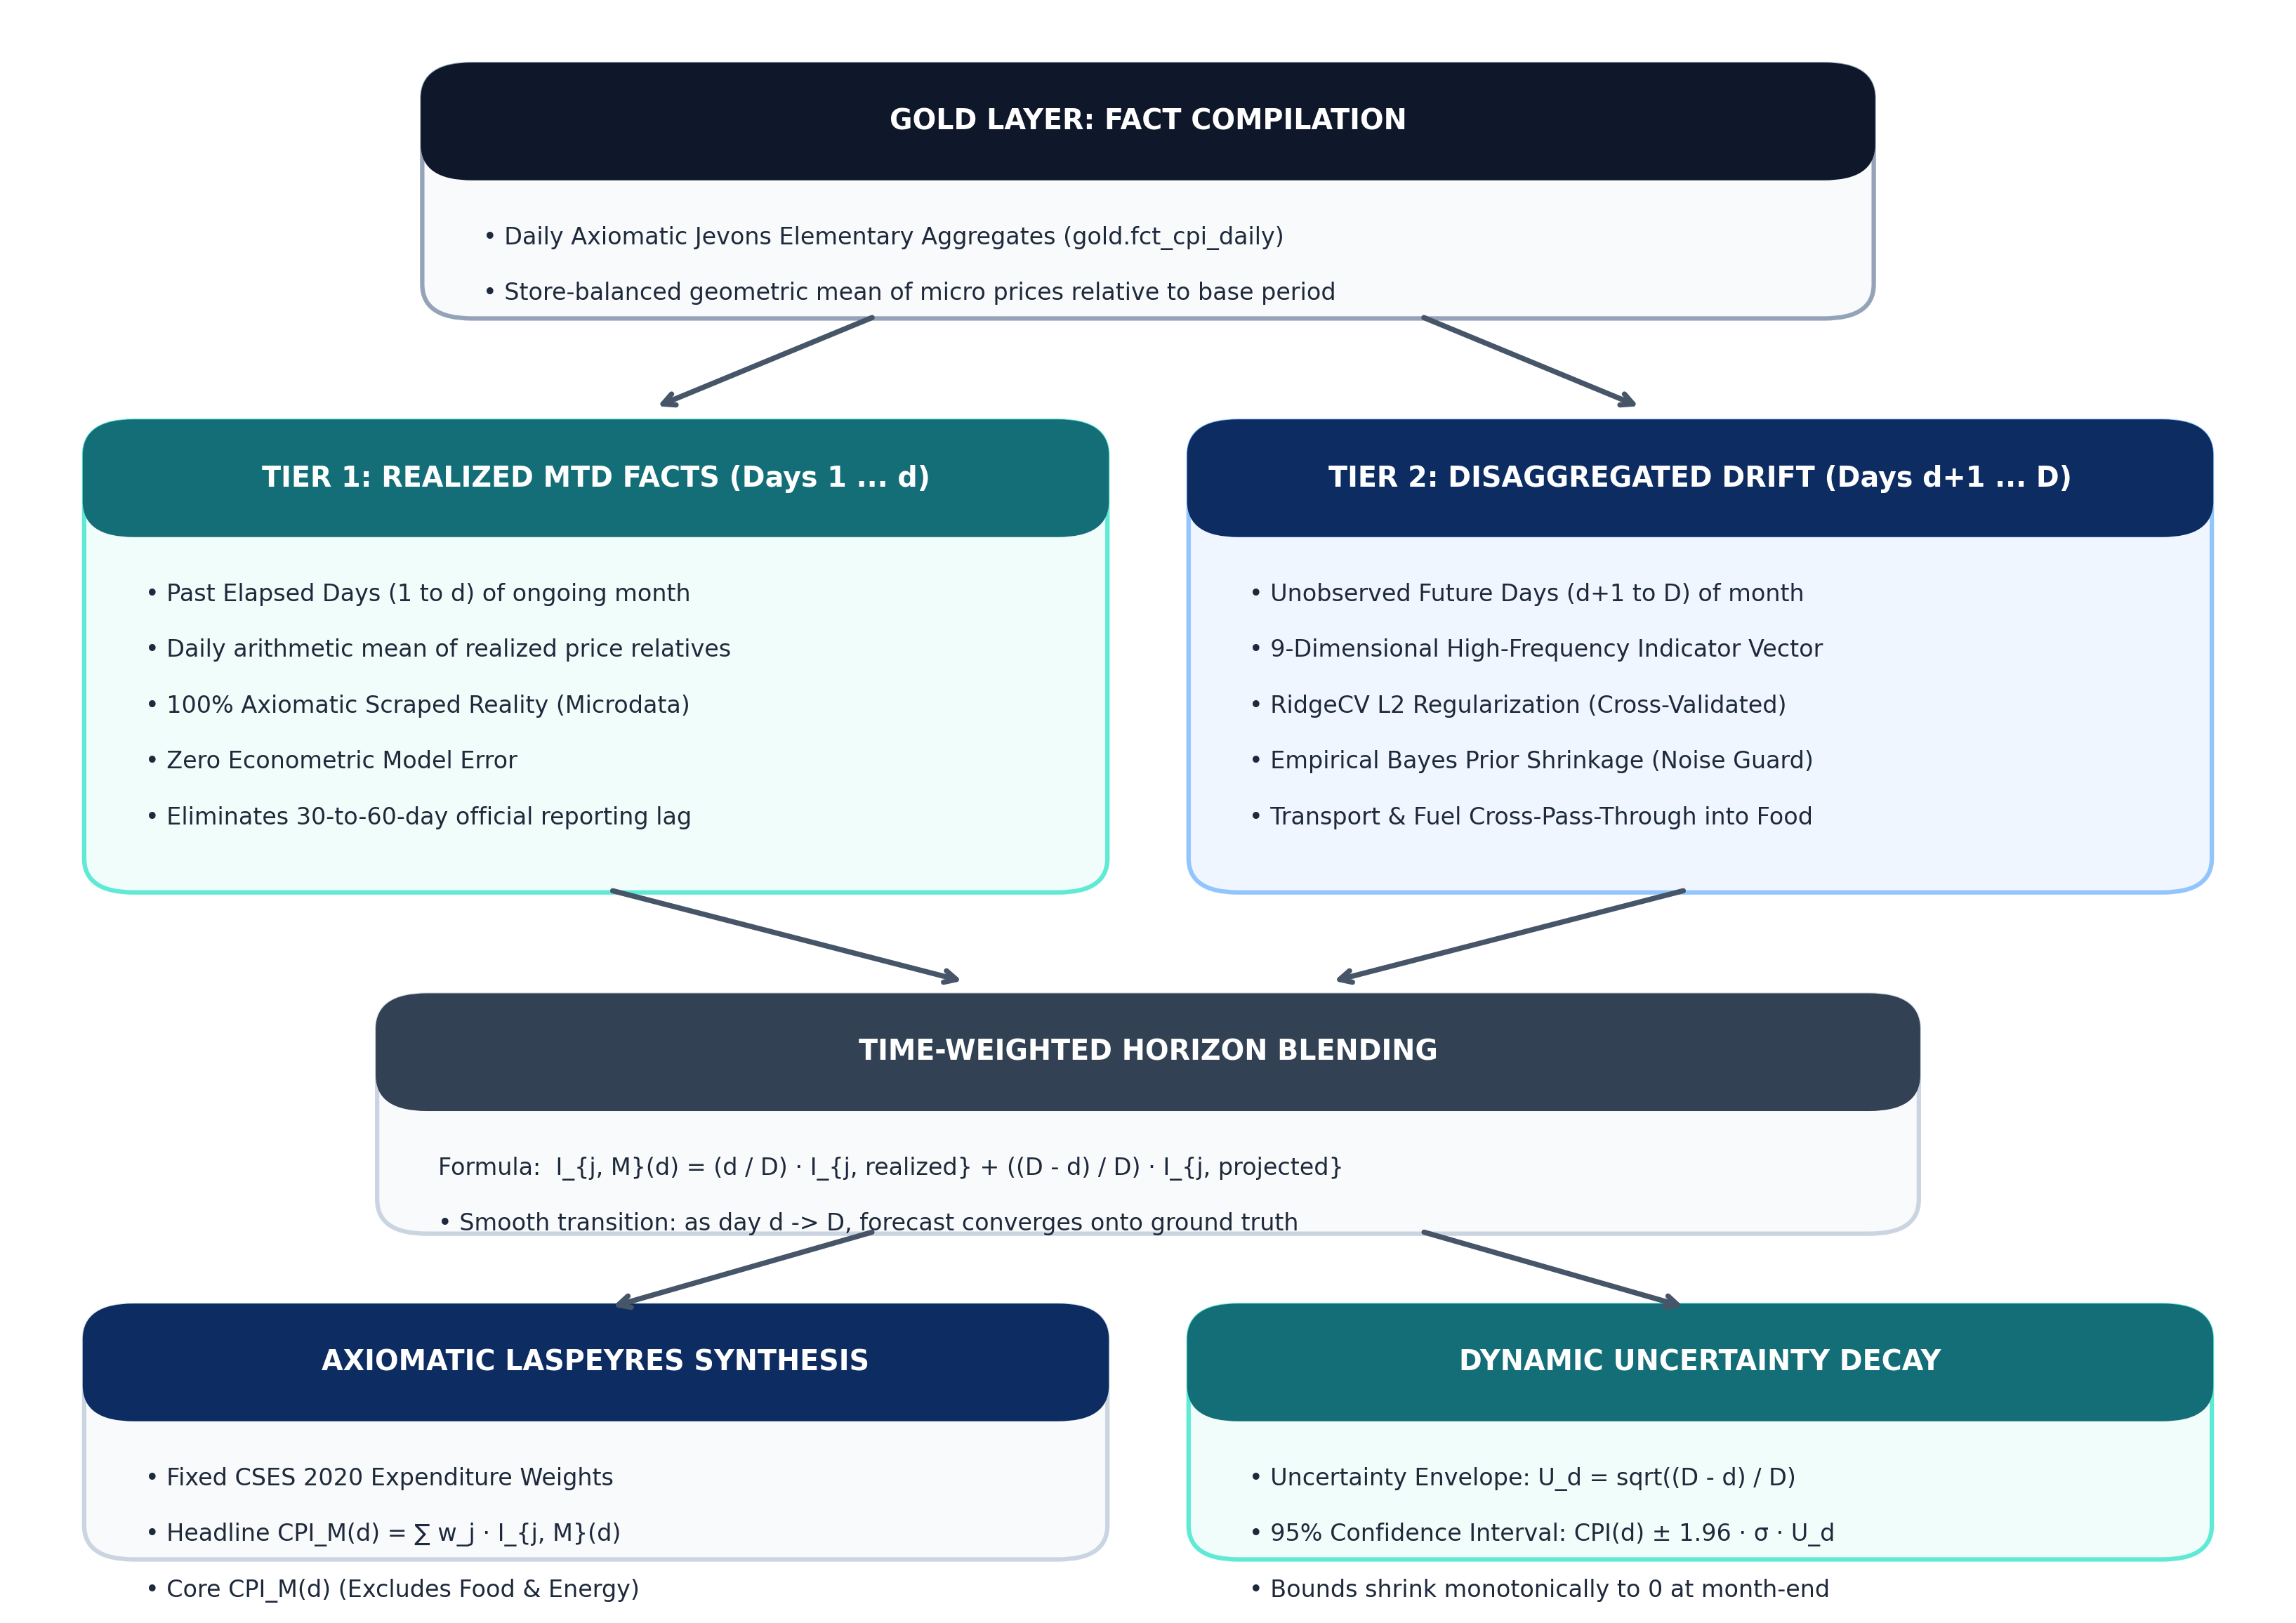
\includegraphics[width=0.96\linewidth]{thesis/images/nowcasting_flowchart.png}
    \caption*{Figure 2: Architecture Flowchart of the Two-Tier Inflation Nowcasting Engine}
\end{figure}

\begin{figure}[H]
    \centering
    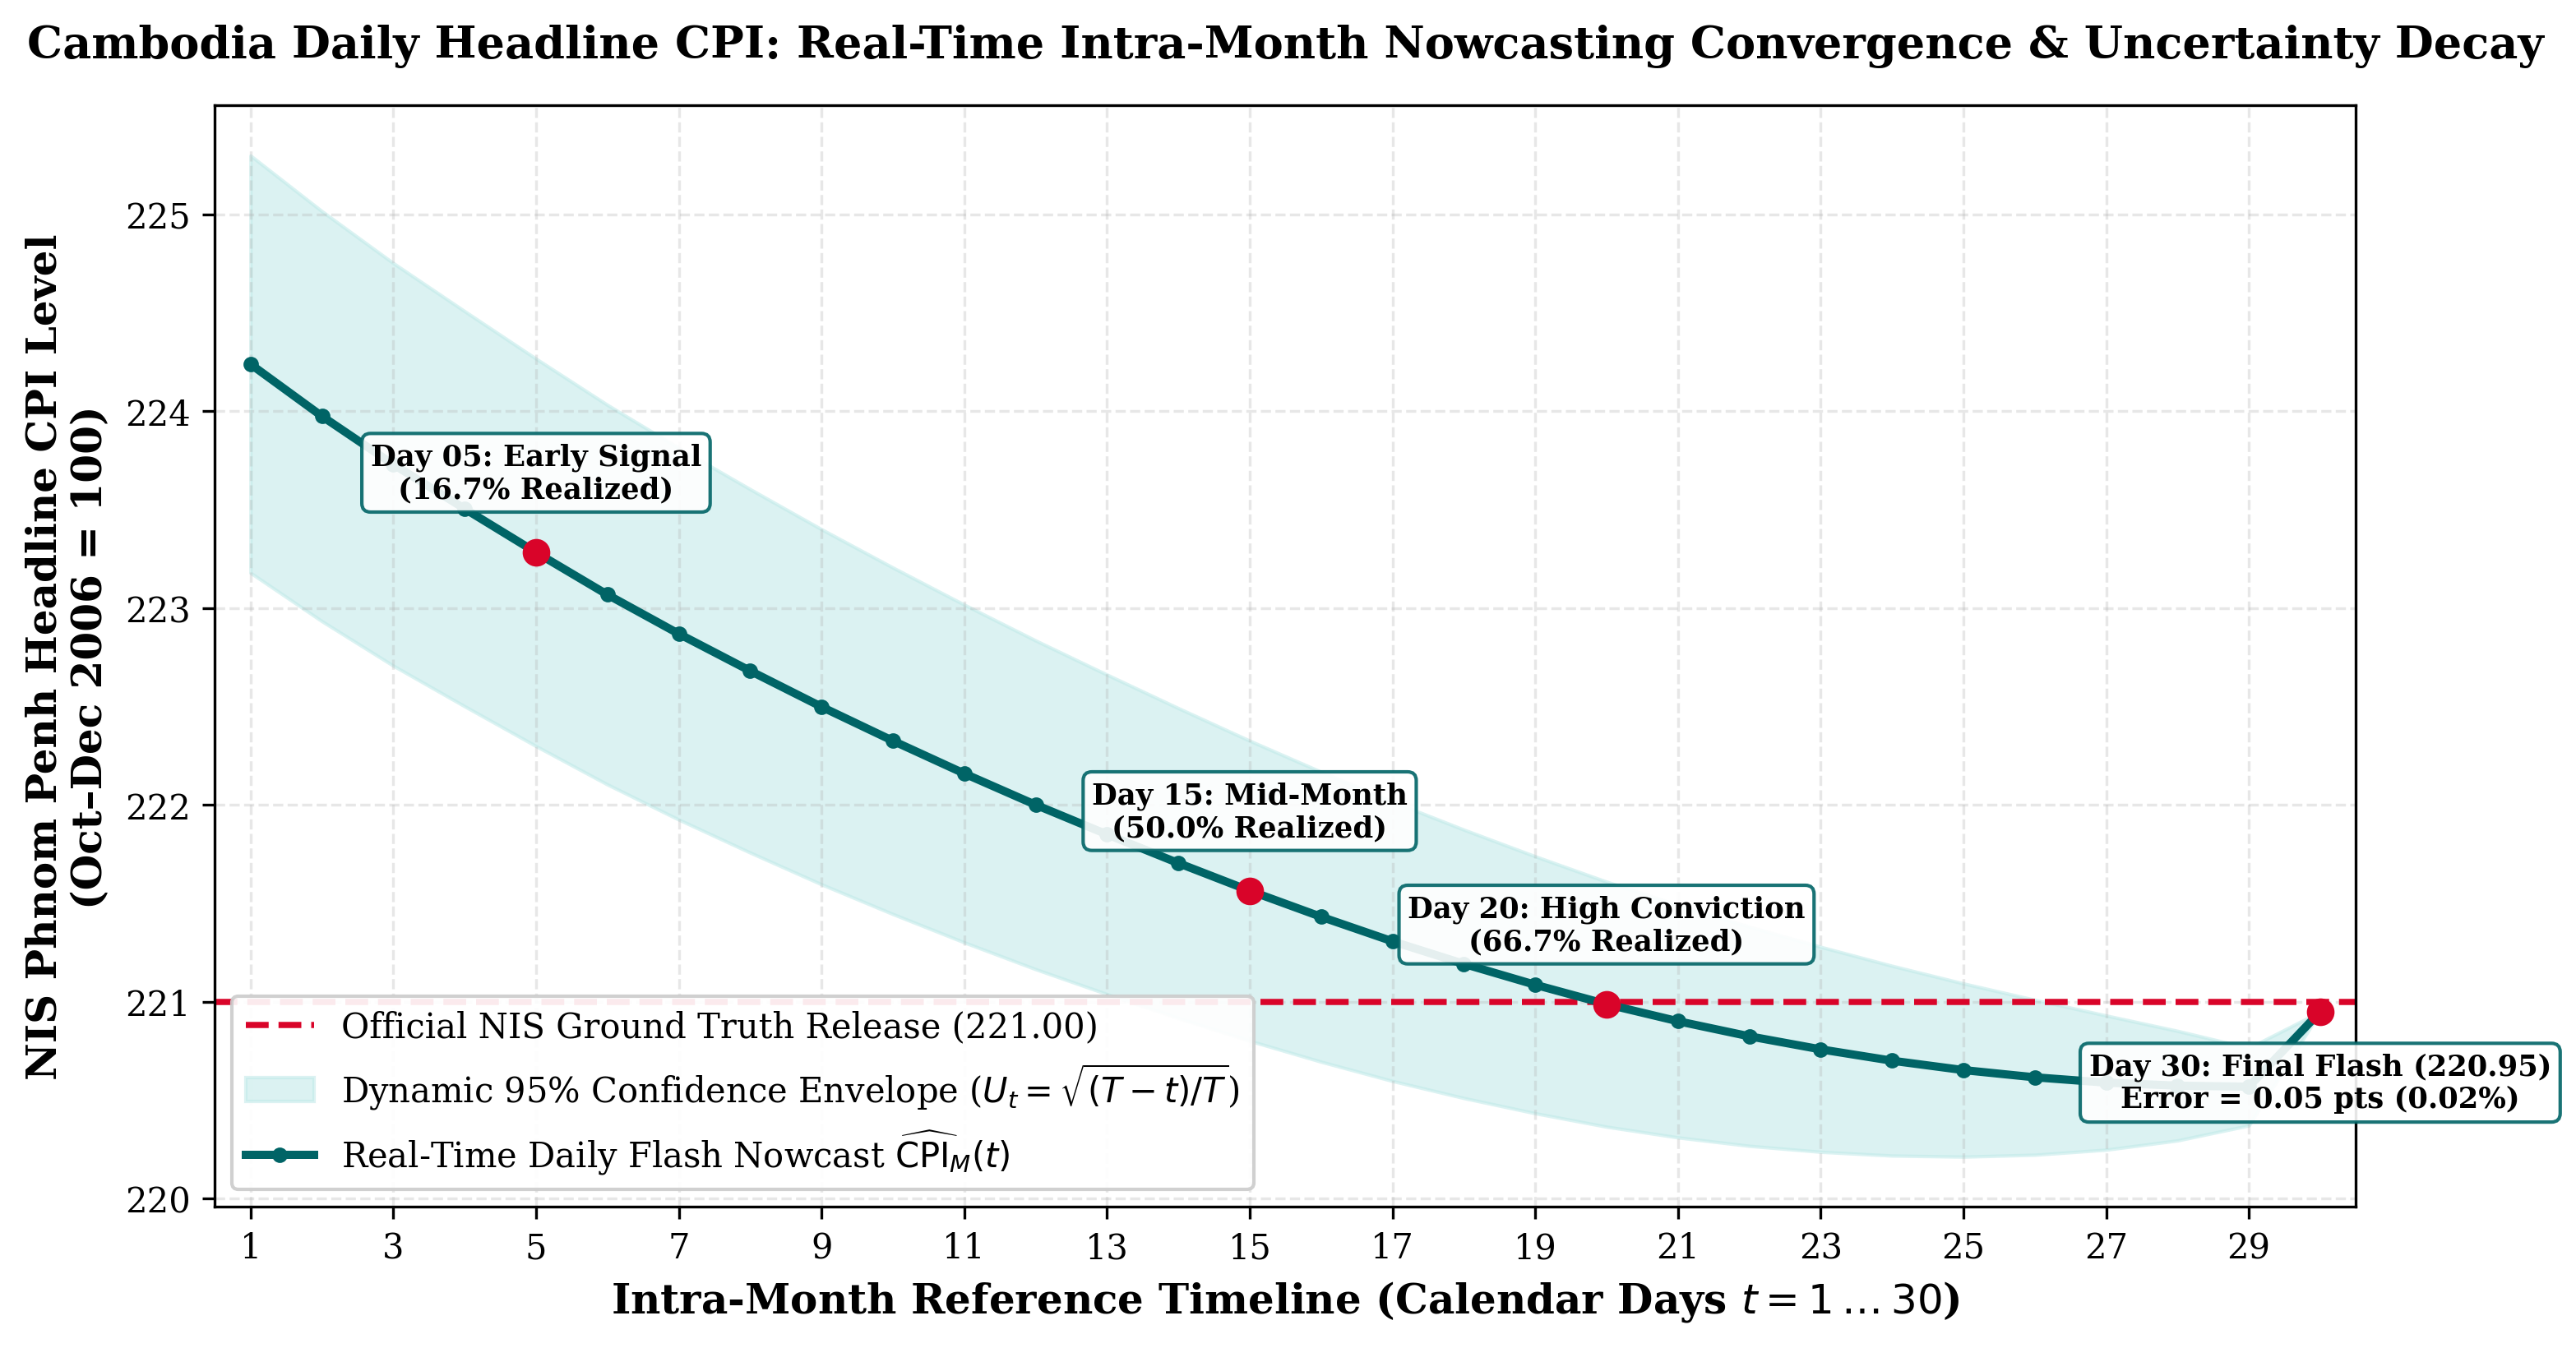
\includegraphics[width=0.92\linewidth]{thesis/images/cpi_nowcasting_convergence.png}
    \caption*{Figure 3: Intra-Month Nowcasting Convergence with Monotonically Decaying Error Bounds}
\end{figure}

\vspace{0.2cm}
\section*{5. Decision-Support Metabase Dashboards \& Monitoring}
\noindent
To provide actionable macroeconomic intelligence and continuous pipeline observability, the system implements three dedicated production dashboards in Metabase (deployed via Docker containers):

\subsection*{Dashboard 1: Macro CPI \& Inflation Analytics}
\noindent
Shows daily Headline CPI and Core CPI (which removes volatile food and fuel prices), monthly inflation rates, and price changes across all 12 consumption categories compared against official government reports.
\begin{figure}[H]
    \centering
    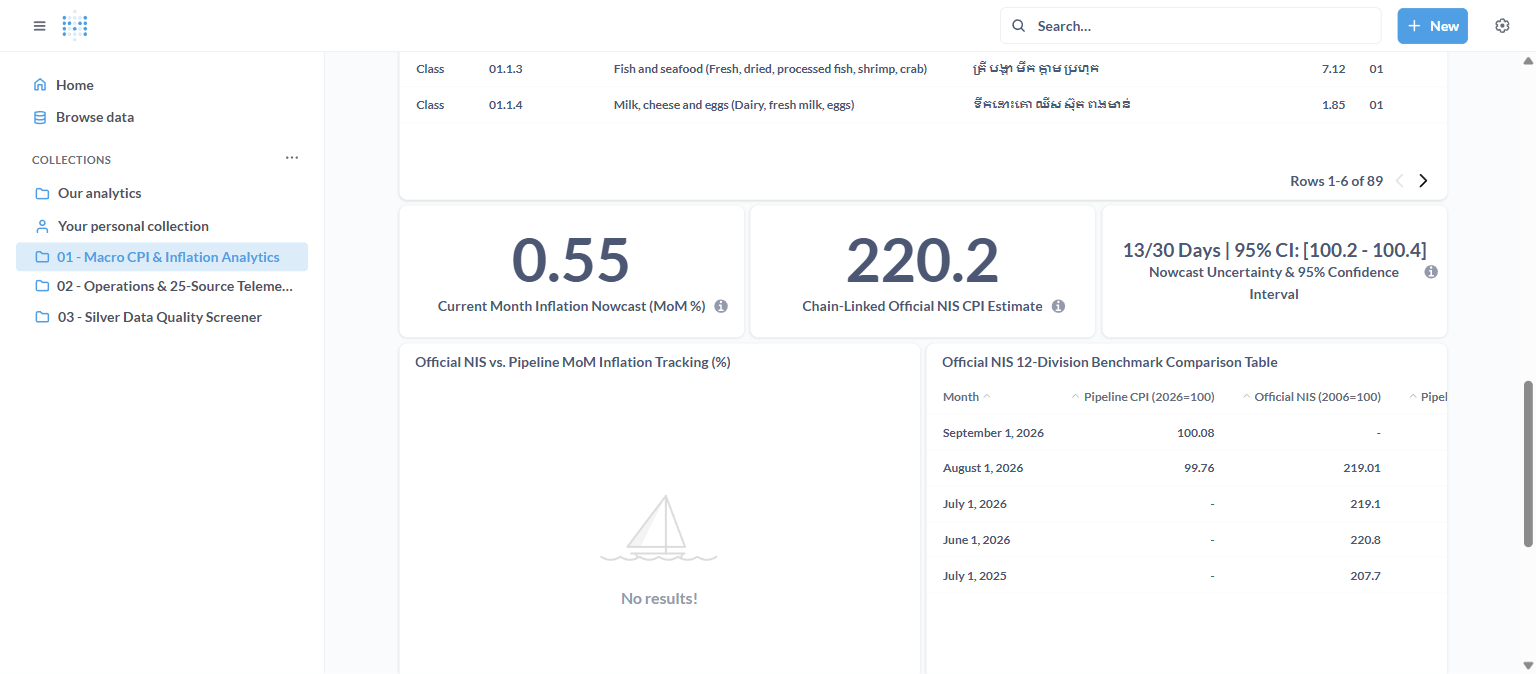
\includegraphics[width=0.95\linewidth]{thesis/images/dashboard_97_macro_cpi.png}
    \caption*{Figure 4: Metabase Dashboard 1 --- Real-Time Macro CPI \& Inflation Analytics}
\end{figure}

\subsection*{Dashboard 2: Operations \& Data Source Telemetry}
\noindent
Tracks the daily health of our scrapers across all 11 sources. It shows how many product prices were collected each day, scraping speed, and website connection status.
\begin{figure}[H]
    \centering
    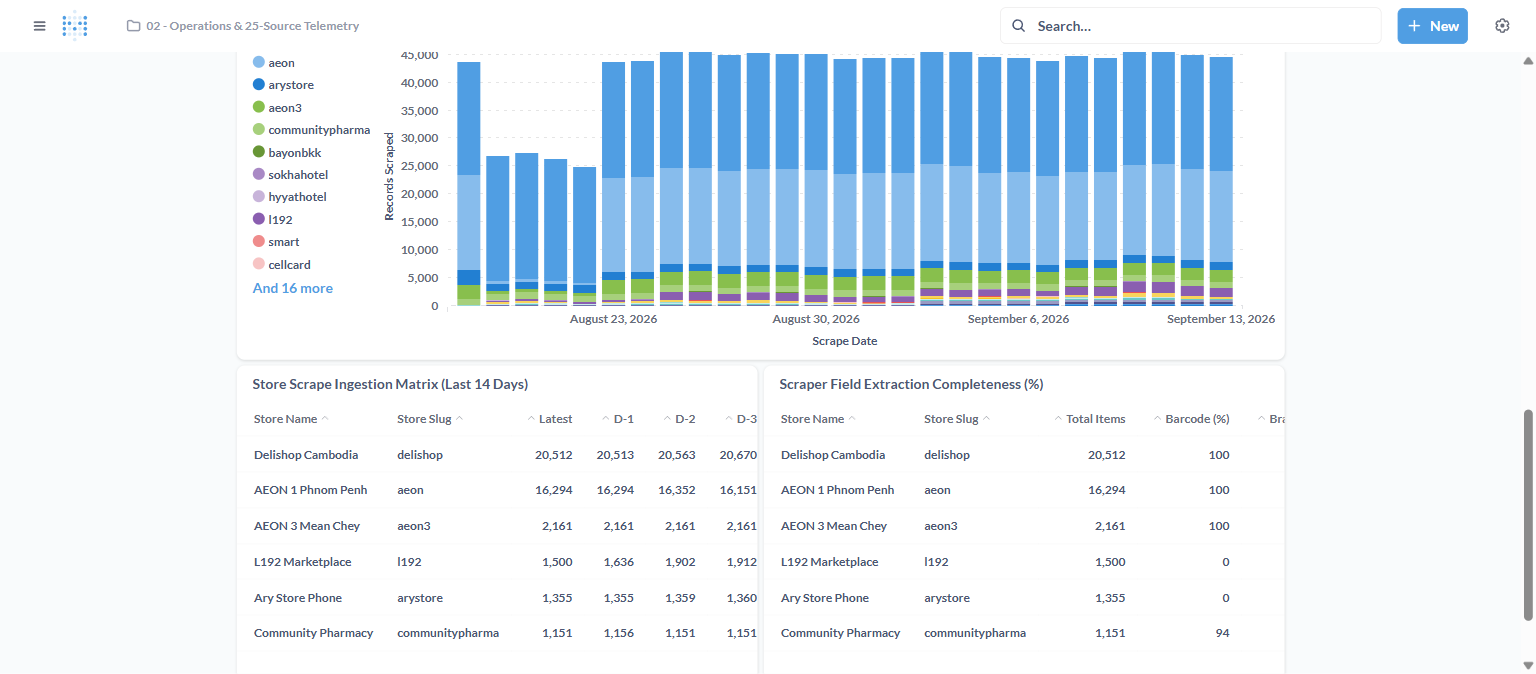
\includegraphics[width=0.95\linewidth]{thesis/images/dashboard_98_telemetry.png}
    \caption*{Figure 5: Metabase Dashboard 2 --- Data Lake Operations \& Scraping Telemetry}
\end{figure}

\subsection*{Dashboard 3: Silver Layer Data Quality Screener}
\noindent
Checks the cleanliness of our data every day. It tracks product size standardization (converting items to 1kg or 1L), USD to Khmer Riel currency conversion, product matching across stores, and AI classification accuracy.
\begin{figure}[H]
    \centering
    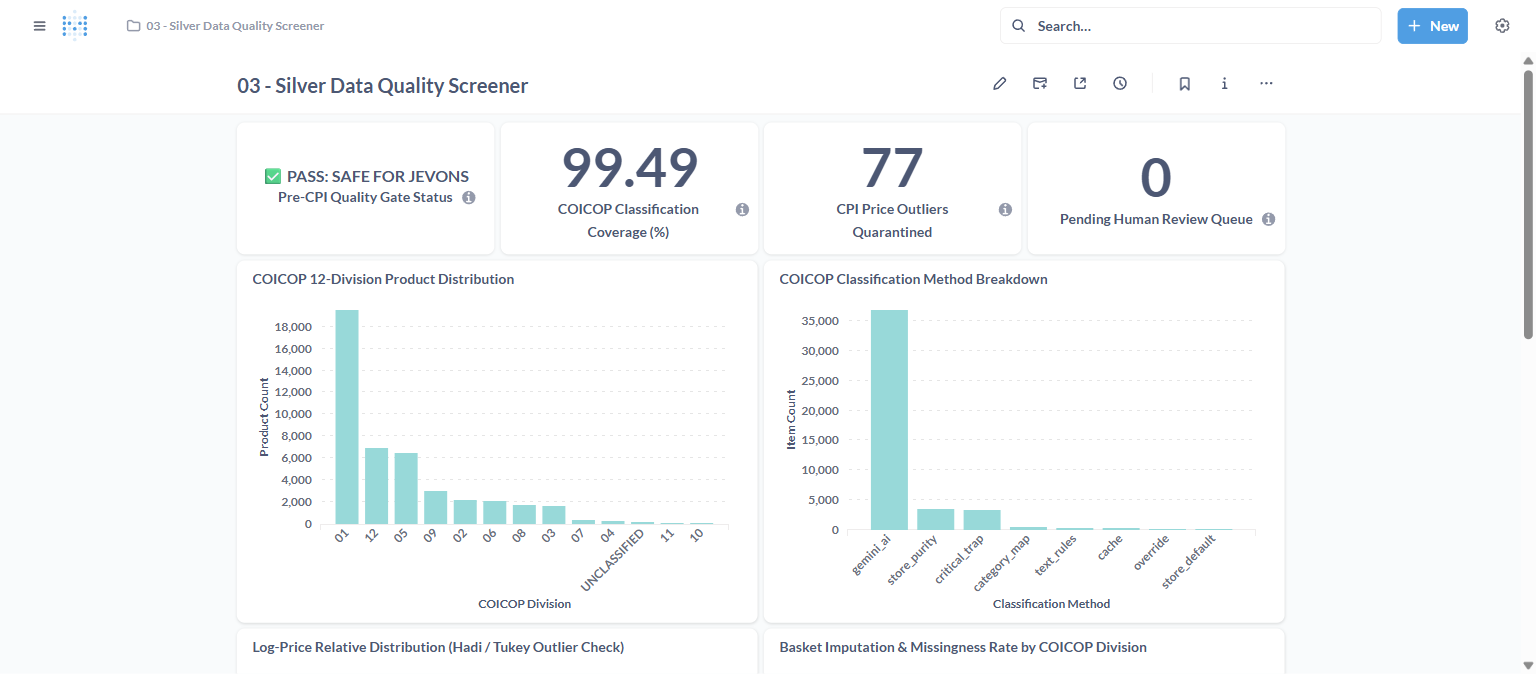
\includegraphics[width=0.95\linewidth]{thesis/images/dashboard_99_silver_quality.png}
    \caption*{Figure 6: Metabase Dashboard 3 --- Silver Layer Data Quality \& Classification Screener}
\end{figure}

\end{document}
